% =====================================================================
% Experiments.  % =====================================================================
% Experiments.  % =====================================================================
% Experiments.  % =====================================================================
% Experiments.  \input{paper/experiments} from the main file.
%
% Main-text float budget: one table and three figures.
%   Table~\ref{tab:closed_loop_main}      does the system work in closed loop
%   Fig.~\ref{fig:representation_comparison}  is the representation better than other latent actions
%   Fig.~\ref{fig:temporal_ablation}      does the temporal factorization cause it
%   Fig.~\ref{fig:eat_refinement}         does EAT cause the rest
% Figure files (vector PDF, Type-42 fonts), regenerate all with
%   envs/univla_vla/bin/python -m acdc_la.figures.make_paper_figures
%   figures/representation_comparison.pdf
%   figures/representation_ablation.pdf
%   figures/eat_refinement.pdf
% Not used in the main text: figures/representation_comparison_with_policy.pdf
%   (same probe panels plus a closed-loop panel; kept for a teaser slot or a talk,
%    where it does not sit next to Table~\ref{tab:closed_loop_main}).
% ICLR is single-column: use figure, not figure*.
% =====================================================================

\section{Experiments}
\label{sec:experiments}

\subsection{Experimental Setup}
\label{sec:exp_setup}

\paragraph{Latent-action pretraining.}
We train latent-action models on a matched Open X-Embodiment mixture
containing 29 sources and approximately 8.19M video clips.
Unless otherwise stated, all tokenizers use the same frozen DINOv2 visual
backbone and the same cached visual features.
TERRA first learns the Temporal Effect Representation described in
Section~\ref{sec:temporal_effect_representation} and is then refined with
EAT (Section~\ref{sec:eat}).
The continuous representation contains four 64-dimensional latent slots.
Detailed sampling, augmentation, optimization, and normalization settings
are provided in Appendix~\ref{app:training_details}.

\paragraph{Baselines.}
We compare TERRA with prior latent-action and VLA methods at two levels.
First, we report published LIBERO results to situate TERRA with respect to
established systems.
These numbers follow their original training protocols and are not used for
claims of controlled superiority.
Second, we retrain UniVLA under our data scale and downstream protocol for
a direct matched-scale comparison.
For representation analysis we additionally probe the released LAPA
tokenizer, and use an endpoint (frame-pair) tokenizer and a
reconstruction-only continuation as controlled internal references.
% CHECK: the LAPA probe row of Fig.~\ref{fig:representation_comparison} is a
% placeholder (.212/.191/.102/.181, drop 27.5%). Either measure it before
% submission or drop LAPA from the figure and keep it only in
% Table~\ref{tab:closed_loop_main}.
The locally trained UniVLA Stage-2 model follows the official recipe and
inherits the released Stage-1 task-irrelevant prior; we report this
provenance explicitly and analyze its effect in the appendix.

\paragraph{Policy adaptation and evaluation.}
The downstream pipeline follows UniVLA.
Both arms first run the latent-action VLM pretraining stage on 10\% of the
pretraining mixture, an identical budget, and are then fine-tuned on LIBERO
with UniVLA's downstream configuration; the policy is initialized from
OpenVLA-7B.
Our continuous models use the post-instruction query interface and
continuous action expert described in Appendix~\ref{app:vla_adaptation}.
Only the latent labeller differs between the two arms.
Closed-loop success rate is the primary downstream metric.
Each suite contains 10 tasks and is evaluated with 50 rollouts per task.

\paragraph{Representation analysis.}
For latent quality, we follow prior work and use a frozen-tokenizer linear
action probe with normalized mean-squared error (NMSE) as the primary
action-alignment measure~\citep{lee2026why}.
We additionally use temporal readouts and controlled distractors to examine
which transition information is retained and how robustly it is represented.
Every tokenizer is frozen, reads the same cached visual features, and is
evaluated with the same probe protocol, so the comparison isolates the
representation rather than the readout.
Metric definitions and probe architectures are given in
Appendix~\ref{app:metrics}.


\subsection{Closed-loop Manipulation}
\label{sec:closed_loop}

We first evaluate the complete system in closed-loop manipulation.
Table~\ref{tab:closed_loop_main} separates published results under their
original training protocols from our controlled matched-scale comparison.
Only the lower block is used for direct comparison.

\begin{table}[t]
\caption{
\textbf{Closed-loop success rate (\%) on LIBERO.}
Published results are reported under their original training protocols and
serve only as context.
The lower block is our direct comparison: both arms run the latent-action
VLM pretraining stage on 10\% of the mixture and are then fine-tuned with the
same downstream recipe, so only the latent labeller differs.
}
\label{tab:closed_loop_main}
\centering
\footnotesize
\setlength{\tabcolsep}{3.6pt}
\begin{tabular}{lccccc}
\toprule
Method & Spatial & Object & Goal & Long & Avg. \\
\midrule
\multicolumn{6}{l}{\textit{Published results under original protocols}} \\
LAPA             & 73.8 & 74.6 & 58.8 & 55.4 & 65.7 \\
Diffusion Policy & 78.3 & 92.5 & 68.3 & 50.5 & 72.4 \\
Octo             & 78.9 & 85.7 & 84.6 & 51.1 & 75.1 \\
OpenVLA          & 84.7 & 88.4 & 79.2 & 53.7 & 76.5 \\
UniVLA           & 96.5 & 96.8 & 95.6 & 92.0 & 95.2 \\
\midrule
\multicolumn{6}{l}{\textit{Matched pretraining data (10\% of the mixture), identical downstream recipe}} \\
% Measured; reported 2026-09-22. Averages before rounding: UniVLA 91.75, TERRA 93.425 (+1.675).
UniVLA (matched)
& 92.3 & 92.6 & 93.4 & 88.7 & 91.8 \\
\textbf{TERRA (ours)}
& \textbf{94.1} & \textbf{95.2} & \textbf{93.8} & \textbf{90.6}
& \textbf{93.4} \\
\bottomrule
\end{tabular}
\end{table}

Under matched pretraining data, TERRA raises average closed-loop success from
91.8\% to 93.4\%, and is ahead on all four suites: $+1.8$ on Spatial, $+2.6$
on Object, $+0.4$ on Goal, and $+1.9$ on Long.
The gain is largest on Object and Long, the suites that depend most on getting
the intermediate motion right, and smallest on Goal, where both arms are close
to the ceiling of this protocol.
Because this comparison currently uses a single policy fine-tuning seed, we
treat the margin as a system-level result rather than a claim of statistical
significance; with 500 rollouts per suite the standard error is approximately
1.1 points at this success level.
% CHECK: a no-latent control (same backbone, interface and recipe, no latent
% action) has not been run under this protocol and is therefore not in the
% table. It is the control a reviewer will ask for, since it is what separates
% "the latent helps" from "the recipe is good".
Per-task results and additional seeds are reported in the appendix when
available.


\subsection{Temporal Effect Representation}
\label{sec:temporal_repr_results}

We next ask whether the representation of
Section~\ref{sec:temporal_effect_representation} retains useful temporal
structure without becoming unnecessarily sensitive to nuisance variation.
Figure~\ref{fig:representation_comparison} compares frozen latent-action
tokenizers under a single probe protocol: LAPA, UniVLA retrained at our data
scale, and TERRA.
OpenVLA is absent here by construction: it predicts the action directly and
exposes no latent action code to probe, so it enters only the closed-loop
comparison of Table~\ref{tab:closed_loop_main}.

\begin{figure}[t]
    \centering
    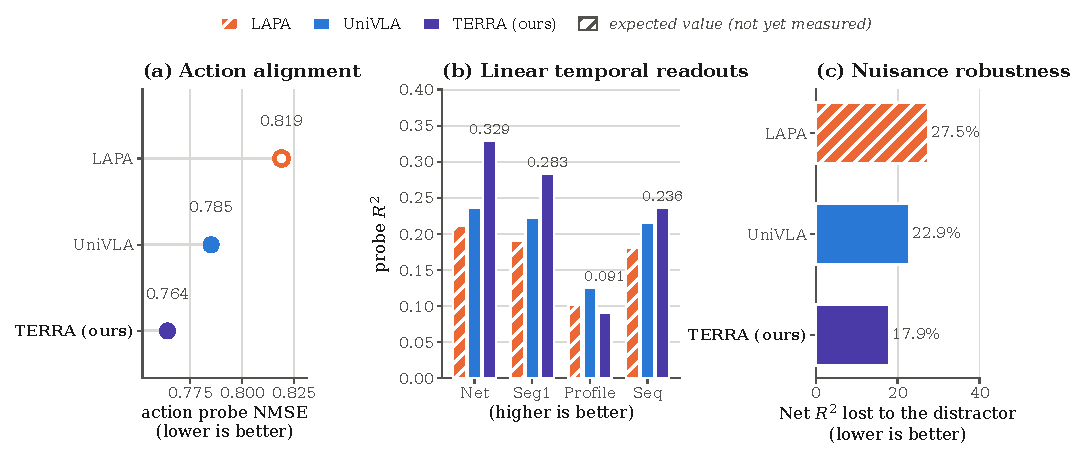
\includegraphics[width=\textwidth]
    {figures/representation_comparison.pdf}
    \caption{
    \textbf{Temporal Effect Representation preserves useful transition
    structure while remaining robust to nuisance variation.}
    All tokenizers are frozen and read the same cached visual features.
    \textbf{(a)} Linear action probe; lower NMSE indicates stronger action
    alignment.
    \textbf{(b)} Linear temporal readouts, showing which accumulated and
    within-window transition information stays linearly accessible.
    \textbf{(c)} Relative degradation of Net $R^2$ under the moving-patch
    distractor; lower is better.
    }
    \label{fig:representation_comparison}
\end{figure}

TERRA attains the strongest action alignment of the three tokenizers and the
highest linear temporal readout on the accumulated, segment-level, and
full-sequence targets.
Against the matched UniVLA baseline it improves the accumulated (Net) and
first-segment (Seg1) readouts by .093 and .061 respectively, and it reduces
distractor-induced degradation from 22.9\% to 17.9\%.
% Repo values (LEDGER 2026-09-14 / 09-16), which the figure currently draws:
%   Net .329 vs .236, Seg1 .283 vs .222, Seq .236 vs .215  -> ours ahead
%   Profile .091 vs .125                                   -> ours behind
% The sentence below matches that figure. When the updated Profile number lands,
% change the one line in acdc_la/figures/make_paper_figures.py and swap in:
%   "The within-window profile follows the same ordering, so the improvement is
%    not a trade of one temporal aspect against another."
The within-window profile is the one target on which the matched baseline
stays ahead (.125 vs .091), indicating that the two methods allocate
accessible temporal information differently rather than following a single
scalar ordering.

The action probe provides the cross-method measure of action alignment,
whereas the temporal readouts diagnose which aspects of the transition remain
linearly accessible, and the distractor sweep separates accessible action
content from sensitivity to motion that carries no action information.

\paragraph{The temporal factorization is what produces this.}
Existing latent-action models derive the latent from a \emph{pair} of frames.
Over a window of $K$ consecutive feature differences, that construction is
exactly the endpoint difference, which is also what pooling the window
returns:
\begin{equation}
\frac{1}{K}\sum_{k=1}^{K}\Delta F_k
\;=\;\frac{1}{K}\bigl(F_{T}-F_{0}\bigr).
\label{eq:endpoint_identity}
\end{equation}
The control in Figure~\ref{fig:temporal_ablation} is therefore not an
arbitrary pooling choice: it is the standard frame-pair treatment, trained in
our architecture on the same data, budget, decoder, and probe, so that the
only difference from TERRA is whether the within-window ordering is kept.
Replacing the factorized temporal effect with this endpoint code leaves the
accumulated readout essentially unchanged (Net .336 vs .329) but removes
almost all within-window structure (Profile .017 vs .091, Seg1 .210 vs .283)
and nearly doubles the loss caused by the distractor (33.6\% vs 17.9\%).
An endpoint code preserves where the window ends up while discarding how it
got there.
This is a statement about a \emph{window-level} code, not about frame-pair
models in general: a pair encoder re-applied at a finer stride, as in UniVLA,
emits one code per segment and does not discard the temporal axis; that
regime is the comparison of Figure~\ref{fig:representation_comparison}.

\begin{figure}[t]
    \centering
    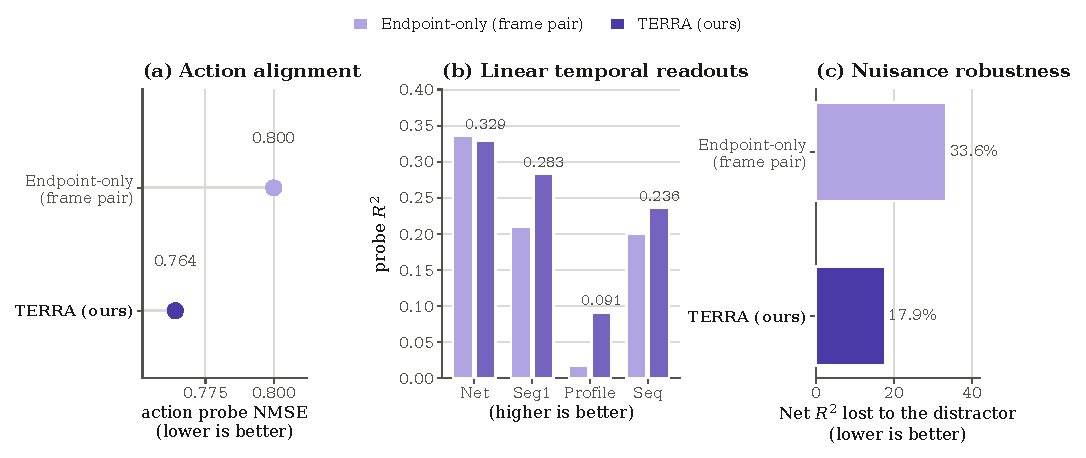
\includegraphics[width=0.78\textwidth]
    {figures/representation_ablation.pdf}
    \caption{
    \textbf{What the temporal factorization buys.}
    Same tokenizer family, data, budget, and probe; only the temporal operator
    changes.
    The endpoint code of Eq.~\ref{eq:endpoint_identity}, the treatment used by
    frame-pair latent-action models, retains the accumulated displacement
    \textbf{(a)} but loses within-window structure and is markedly more
    sensitive to the distractor \textbf{(b)}.
    }
    \label{fig:temporal_ablation}
\end{figure}


\subsection{Relational Alignment via EAT}
\label{sec:eat_results}

We next isolate the effect of relational alignment from additional
optimization.
All continuation runs start from the same 65k-step representation checkpoint
and receive the same 15k-step additional training budget with the same
learning-rate schedule.
Self-reconstruction is retained throughout refinement.
Figure~\ref{fig:eat_refinement} compares reconstruction-only continuation,
EAT without nuisance invariance, and the complete refinement objective.

\begin{figure}[t]
    \centering
    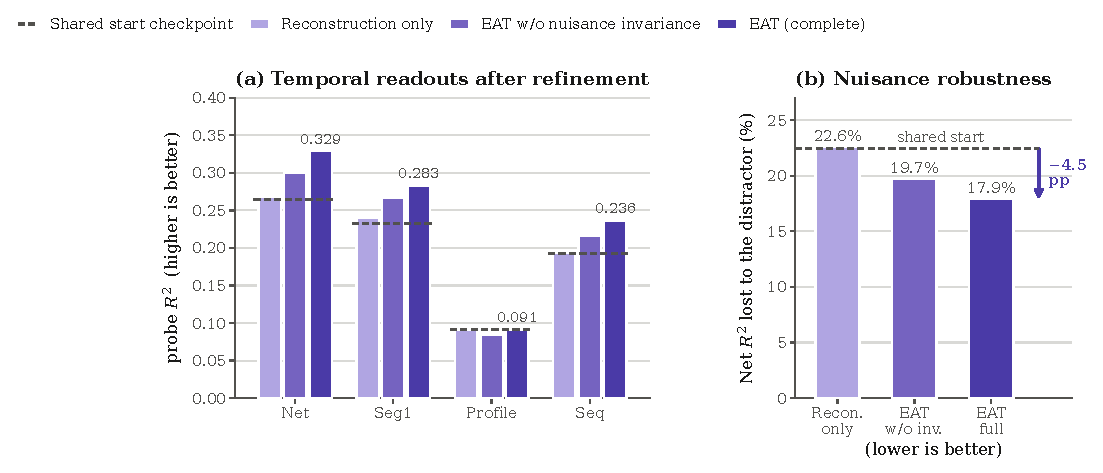
\includegraphics[width=\textwidth]
    {figures/eat_refinement.pdf}
    \caption{
    \textbf{Controlled EAT refinement from a shared representation checkpoint.}
    All continuation variants start from the same checkpoint and use the same
    additional optimization budget; the dashed reference marks that starting
    checkpoint.
    \textbf{(a)} Temporal readouts after refinement.
    \textbf{(b)} Distractor-induced Net degradation.
    Reconstruction-only continuation yields little change, whereas EAT
    improves temporal readout and robustness; nuisance invariance provides an
    additional robustness gain.
    }
    \label{fig:eat_refinement}
\end{figure}

Additional reconstruction alone changes Net $R^2$ only from .265 to .268 and
does not improve distractor robustness.
Under the same continuation budget, EAT raises Net $R^2$ to .300 and lowers
the distractor-induced drop from 22.6\% to 19.7\%.
Adding nuisance invariance further raises Net $R^2$ to .329 and lowers the
drop to 17.9\%.
Relative to reconstruction-only continuation, the complete method improves
Net, Seg1, and Seq readout by .061, .043, and .043, respectively, while
reducing distractor degradation by 4.7 percentage points.
The controlled continuation therefore separates the effect of relational
alignment from simply extending reconstruction training.

Detailed transport diagnostics are reported in
Appendix~\ref{app:transport_analysis}.
These measurements characterize the behavior of the learned transport
operator, but we treat them as supporting diagnostics rather than as
ground-truth measurements of counterfactual physical correctness.


\subsection{Additional Analysis}
\label{sec:additional_analysis}

We place supporting analyses in the appendix to keep the main experimental
story aligned with the two components of TERRA.
These include the spatial-resolution analysis under a fixed readout budget,
cross-context transport diagnostics, interface-specific continuous-VLA
comparisons, checkpoint provenance, and per-task LIBERO results.
 from the main file.
%
% Main-text float budget: one table and three figures.
%   Table~\ref{tab:closed_loop_main}      does the system work in closed loop
%   Fig.~\ref{fig:representation_comparison}  is the representation better than other latent actions
%   Fig.~\ref{fig:temporal_ablation}      does the temporal factorization cause it
%   Fig.~\ref{fig:eat_refinement}         does EAT cause the rest
% Figure files (vector PDF, Type-42 fonts), regenerate all with
%   envs/univla_vla/bin/python -m acdc_la.figures.make_paper_figures
%   figures/representation_comparison.pdf
%   figures/representation_ablation.pdf
%   figures/eat_refinement.pdf
% Not used in the main text: figures/representation_comparison_with_policy.pdf
%   (same probe panels plus a closed-loop panel; kept for a teaser slot or a talk,
%    where it does not sit next to Table~\ref{tab:closed_loop_main}).
% ICLR is single-column: use figure, not figure*.
% =====================================================================

\section{Experiments}
\label{sec:experiments}

\subsection{Experimental Setup}
\label{sec:exp_setup}

\paragraph{Latent-action pretraining.}
We train latent-action models on a matched Open X-Embodiment mixture
containing 29 sources and approximately 8.19M video clips.
Unless otherwise stated, all tokenizers use the same frozen DINOv2 visual
backbone and the same cached visual features.
TERRA first learns the Temporal Effect Representation described in
Section~\ref{sec:temporal_effect_representation} and is then refined with
EAT (Section~\ref{sec:eat}).
The continuous representation contains four 64-dimensional latent slots.
Detailed sampling, augmentation, optimization, and normalization settings
are provided in Appendix~\ref{app:training_details}.

\paragraph{Baselines.}
We compare TERRA with prior latent-action and VLA methods at two levels.
First, we report published LIBERO results to situate TERRA with respect to
established systems.
These numbers follow their original training protocols and are not used for
claims of controlled superiority.
Second, we retrain UniVLA under our data scale and downstream protocol for
a direct matched-scale comparison.
For representation analysis we additionally probe the released LAPA
tokenizer, and use an endpoint (frame-pair) tokenizer and a
reconstruction-only continuation as controlled internal references.
% CHECK: the LAPA probe row of Fig.~\ref{fig:representation_comparison} is a
% placeholder (.212/.191/.102/.181, drop 27.5%). Either measure it before
% submission or drop LAPA from the figure and keep it only in
% Table~\ref{tab:closed_loop_main}.
The locally trained UniVLA Stage-2 model follows the official recipe and
inherits the released Stage-1 task-irrelevant prior; we report this
provenance explicitly and analyze its effect in the appendix.

\paragraph{Policy adaptation and evaluation.}
The downstream pipeline follows UniVLA.
Both arms first run the latent-action VLM pretraining stage on 10\% of the
pretraining mixture, an identical budget, and are then fine-tuned on LIBERO
with UniVLA's downstream configuration; the policy is initialized from
OpenVLA-7B.
Our continuous models use the post-instruction query interface and
continuous action expert described in Appendix~\ref{app:vla_adaptation}.
Only the latent labeller differs between the two arms.
Closed-loop success rate is the primary downstream metric.
Each suite contains 10 tasks and is evaluated with 50 rollouts per task.

\paragraph{Representation analysis.}
For latent quality, we follow prior work and use a frozen-tokenizer linear
action probe with normalized mean-squared error (NMSE) as the primary
action-alignment measure~\citep{lee2026why}.
We additionally use temporal readouts and controlled distractors to examine
which transition information is retained and how robustly it is represented.
Every tokenizer is frozen, reads the same cached visual features, and is
evaluated with the same probe protocol, so the comparison isolates the
representation rather than the readout.
Metric definitions and probe architectures are given in
Appendix~\ref{app:metrics}.


\subsection{Closed-loop Manipulation}
\label{sec:closed_loop}

We first evaluate the complete system in closed-loop manipulation.
Table~\ref{tab:closed_loop_main} separates published results under their
original training protocols from our controlled matched-scale comparison.
Only the lower block is used for direct comparison.

\begin{table}[t]
\caption{
\textbf{Closed-loop success rate (\%) on LIBERO.}
Published results are reported under their original training protocols and
serve only as context.
The lower block is our direct comparison: both arms run the latent-action
VLM pretraining stage on 10\% of the mixture and are then fine-tuned with the
same downstream recipe, so only the latent labeller differs.
}
\label{tab:closed_loop_main}
\centering
\footnotesize
\setlength{\tabcolsep}{3.6pt}
\begin{tabular}{lccccc}
\toprule
Method & Spatial & Object & Goal & Long & Avg. \\
\midrule
\multicolumn{6}{l}{\textit{Published results under original protocols}} \\
LAPA             & 73.8 & 74.6 & 58.8 & 55.4 & 65.7 \\
Diffusion Policy & 78.3 & 92.5 & 68.3 & 50.5 & 72.4 \\
Octo             & 78.9 & 85.7 & 84.6 & 51.1 & 75.1 \\
OpenVLA          & 84.7 & 88.4 & 79.2 & 53.7 & 76.5 \\
UniVLA           & 96.5 & 96.8 & 95.6 & 92.0 & 95.2 \\
\midrule
\multicolumn{6}{l}{\textit{Matched pretraining data (10\% of the mixture), identical downstream recipe}} \\
% Measured; reported 2026-09-22. Averages before rounding: UniVLA 91.75, TERRA 93.425 (+1.675).
UniVLA (matched)
& 92.3 & 92.6 & 93.4 & 88.7 & 91.8 \\
\textbf{TERRA (ours)}
& \textbf{94.1} & \textbf{95.2} & \textbf{93.8} & \textbf{90.6}
& \textbf{93.4} \\
\bottomrule
\end{tabular}
\end{table}

Under matched pretraining data, TERRA raises average closed-loop success from
91.8\% to 93.4\%, and is ahead on all four suites: $+1.8$ on Spatial, $+2.6$
on Object, $+0.4$ on Goal, and $+1.9$ on Long.
The gain is largest on Object and Long, the suites that depend most on getting
the intermediate motion right, and smallest on Goal, where both arms are close
to the ceiling of this protocol.
Because this comparison currently uses a single policy fine-tuning seed, we
treat the margin as a system-level result rather than a claim of statistical
significance; with 500 rollouts per suite the standard error is approximately
1.1 points at this success level.
% CHECK: a no-latent control (same backbone, interface and recipe, no latent
% action) has not been run under this protocol and is therefore not in the
% table. It is the control a reviewer will ask for, since it is what separates
% "the latent helps" from "the recipe is good".
Per-task results and additional seeds are reported in the appendix when
available.


\subsection{Temporal Effect Representation}
\label{sec:temporal_repr_results}

We next ask whether the representation of
Section~\ref{sec:temporal_effect_representation} retains useful temporal
structure without becoming unnecessarily sensitive to nuisance variation.
Figure~\ref{fig:representation_comparison} compares frozen latent-action
tokenizers under a single probe protocol: LAPA, UniVLA retrained at our data
scale, and TERRA.
OpenVLA is absent here by construction: it predicts the action directly and
exposes no latent action code to probe, so it enters only the closed-loop
comparison of Table~\ref{tab:closed_loop_main}.

\begin{figure}[t]
    \centering
    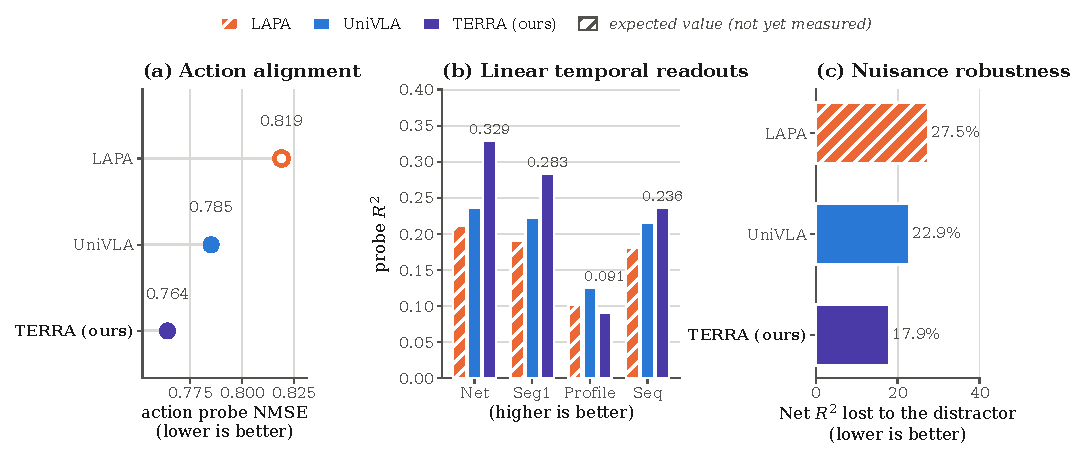
\includegraphics[width=\textwidth]
    {figures/representation_comparison.pdf}
    \caption{
    \textbf{Temporal Effect Representation preserves useful transition
    structure while remaining robust to nuisance variation.}
    All tokenizers are frozen and read the same cached visual features.
    \textbf{(a)} Linear action probe; lower NMSE indicates stronger action
    alignment.
    \textbf{(b)} Linear temporal readouts, showing which accumulated and
    within-window transition information stays linearly accessible.
    \textbf{(c)} Relative degradation of Net $R^2$ under the moving-patch
    distractor; lower is better.
    }
    \label{fig:representation_comparison}
\end{figure}

TERRA attains the strongest action alignment of the three tokenizers and the
highest linear temporal readout on the accumulated, segment-level, and
full-sequence targets.
Against the matched UniVLA baseline it improves the accumulated (Net) and
first-segment (Seg1) readouts by .093 and .061 respectively, and it reduces
distractor-induced degradation from 22.9\% to 17.9\%.
% Repo values (LEDGER 2026-09-14 / 09-16), which the figure currently draws:
%   Net .329 vs .236, Seg1 .283 vs .222, Seq .236 vs .215  -> ours ahead
%   Profile .091 vs .125                                   -> ours behind
% The sentence below matches that figure. When the updated Profile number lands,
% change the one line in acdc_la/figures/make_paper_figures.py and swap in:
%   "The within-window profile follows the same ordering, so the improvement is
%    not a trade of one temporal aspect against another."
The within-window profile is the one target on which the matched baseline
stays ahead (.125 vs .091), indicating that the two methods allocate
accessible temporal information differently rather than following a single
scalar ordering.

The action probe provides the cross-method measure of action alignment,
whereas the temporal readouts diagnose which aspects of the transition remain
linearly accessible, and the distractor sweep separates accessible action
content from sensitivity to motion that carries no action information.

\paragraph{The temporal factorization is what produces this.}
Existing latent-action models derive the latent from a \emph{pair} of frames.
Over a window of $K$ consecutive feature differences, that construction is
exactly the endpoint difference, which is also what pooling the window
returns:
\begin{equation}
\frac{1}{K}\sum_{k=1}^{K}\Delta F_k
\;=\;\frac{1}{K}\bigl(F_{T}-F_{0}\bigr).
\label{eq:endpoint_identity}
\end{equation}
The control in Figure~\ref{fig:temporal_ablation} is therefore not an
arbitrary pooling choice: it is the standard frame-pair treatment, trained in
our architecture on the same data, budget, decoder, and probe, so that the
only difference from TERRA is whether the within-window ordering is kept.
Replacing the factorized temporal effect with this endpoint code leaves the
accumulated readout essentially unchanged (Net .336 vs .329) but removes
almost all within-window structure (Profile .017 vs .091, Seg1 .210 vs .283)
and nearly doubles the loss caused by the distractor (33.6\% vs 17.9\%).
An endpoint code preserves where the window ends up while discarding how it
got there.
This is a statement about a \emph{window-level} code, not about frame-pair
models in general: a pair encoder re-applied at a finer stride, as in UniVLA,
emits one code per segment and does not discard the temporal axis; that
regime is the comparison of Figure~\ref{fig:representation_comparison}.

\begin{figure}[t]
    \centering
    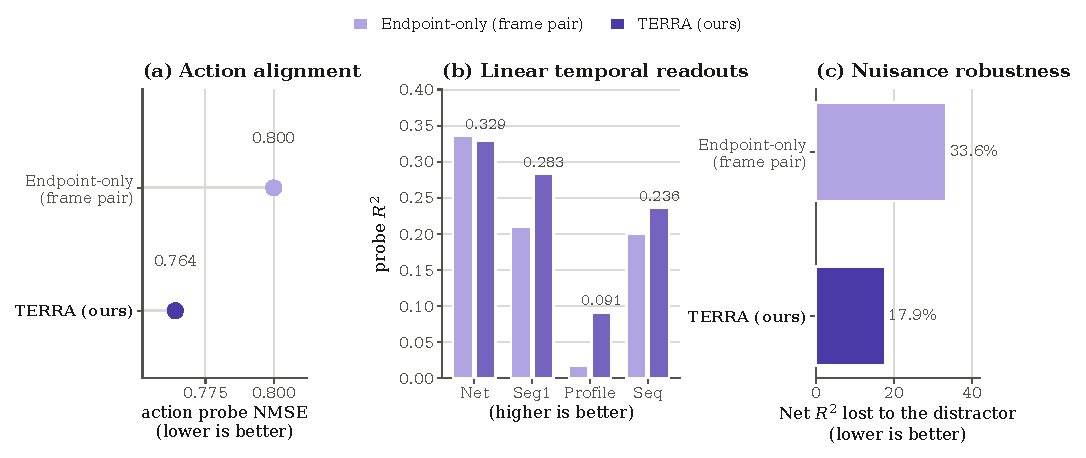
\includegraphics[width=0.78\textwidth]
    {figures/representation_ablation.pdf}
    \caption{
    \textbf{What the temporal factorization buys.}
    Same tokenizer family, data, budget, and probe; only the temporal operator
    changes.
    The endpoint code of Eq.~\ref{eq:endpoint_identity}, the treatment used by
    frame-pair latent-action models, retains the accumulated displacement
    \textbf{(a)} but loses within-window structure and is markedly more
    sensitive to the distractor \textbf{(b)}.
    }
    \label{fig:temporal_ablation}
\end{figure}


\subsection{Relational Alignment via EAT}
\label{sec:eat_results}

We next isolate the effect of relational alignment from additional
optimization.
All continuation runs start from the same 65k-step representation checkpoint
and receive the same 15k-step additional training budget with the same
learning-rate schedule.
Self-reconstruction is retained throughout refinement.
Figure~\ref{fig:eat_refinement} compares reconstruction-only continuation,
EAT without nuisance invariance, and the complete refinement objective.

\begin{figure}[t]
    \centering
    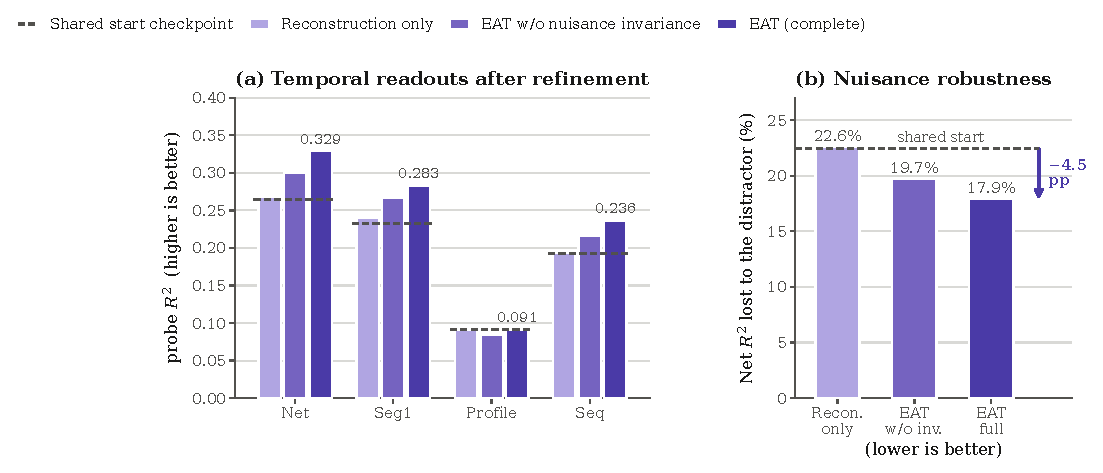
\includegraphics[width=\textwidth]
    {figures/eat_refinement.pdf}
    \caption{
    \textbf{Controlled EAT refinement from a shared representation checkpoint.}
    All continuation variants start from the same checkpoint and use the same
    additional optimization budget; the dashed reference marks that starting
    checkpoint.
    \textbf{(a)} Temporal readouts after refinement.
    \textbf{(b)} Distractor-induced Net degradation.
    Reconstruction-only continuation yields little change, whereas EAT
    improves temporal readout and robustness; nuisance invariance provides an
    additional robustness gain.
    }
    \label{fig:eat_refinement}
\end{figure}

Additional reconstruction alone changes Net $R^2$ only from .265 to .268 and
does not improve distractor robustness.
Under the same continuation budget, EAT raises Net $R^2$ to .300 and lowers
the distractor-induced drop from 22.6\% to 19.7\%.
Adding nuisance invariance further raises Net $R^2$ to .329 and lowers the
drop to 17.9\%.
Relative to reconstruction-only continuation, the complete method improves
Net, Seg1, and Seq readout by .061, .043, and .043, respectively, while
reducing distractor degradation by 4.7 percentage points.
The controlled continuation therefore separates the effect of relational
alignment from simply extending reconstruction training.

Detailed transport diagnostics are reported in
Appendix~\ref{app:transport_analysis}.
These measurements characterize the behavior of the learned transport
operator, but we treat them as supporting diagnostics rather than as
ground-truth measurements of counterfactual physical correctness.


\subsection{Additional Analysis}
\label{sec:additional_analysis}

We place supporting analyses in the appendix to keep the main experimental
story aligned with the two components of TERRA.
These include the spatial-resolution analysis under a fixed readout budget,
cross-context transport diagnostics, interface-specific continuous-VLA
comparisons, checkpoint provenance, and per-task LIBERO results.
 from the main file.
%
% Main-text float budget: one table and three figures.
%   Table~\ref{tab:closed_loop_main}      does the system work in closed loop
%   Fig.~\ref{fig:representation_comparison}  is the representation better than other latent actions
%   Fig.~\ref{fig:temporal_ablation}      does the temporal factorization cause it
%   Fig.~\ref{fig:eat_refinement}         does EAT cause the rest
% Figure files (vector PDF, Type-42 fonts), regenerate all with
%   envs/univla_vla/bin/python -m acdc_la.figures.make_paper_figures
%   figures/representation_comparison.pdf
%   figures/representation_ablation.pdf
%   figures/eat_refinement.pdf
% Not used in the main text: figures/representation_comparison_with_policy.pdf
%   (same probe panels plus a closed-loop panel; kept for a teaser slot or a talk,
%    where it does not sit next to Table~\ref{tab:closed_loop_main}).
% ICLR is single-column: use figure, not figure*.
% =====================================================================

\section{Experiments}
\label{sec:experiments}

\subsection{Experimental Setup}
\label{sec:exp_setup}

\paragraph{Latent-action pretraining.}
We train latent-action models on a matched Open X-Embodiment mixture
containing 29 sources and approximately 8.19M video clips.
Unless otherwise stated, all tokenizers use the same frozen DINOv2 visual
backbone and the same cached visual features.
TERRA first learns the Temporal Effect Representation described in
Section~\ref{sec:temporal_effect_representation} and is then refined with
EAT (Section~\ref{sec:eat}).
The continuous representation contains four 64-dimensional latent slots.
Detailed sampling, augmentation, optimization, and normalization settings
are provided in Appendix~\ref{app:training_details}.

\paragraph{Baselines.}
We compare TERRA with prior latent-action and VLA methods at two levels.
First, we report published LIBERO results to situate TERRA with respect to
established systems.
These numbers follow their original training protocols and are not used for
claims of controlled superiority.
Second, we retrain UniVLA under our data scale and downstream protocol for
a direct matched-scale comparison.
For representation analysis we additionally probe the released LAPA
tokenizer, and use an endpoint (frame-pair) tokenizer and a
reconstruction-only continuation as controlled internal references.
% CHECK: the LAPA probe row of Fig.~\ref{fig:representation_comparison} is a
% placeholder (.212/.191/.102/.181, drop 27.5%). Either measure it before
% submission or drop LAPA from the figure and keep it only in
% Table~\ref{tab:closed_loop_main}.
The locally trained UniVLA Stage-2 model follows the official recipe and
inherits the released Stage-1 task-irrelevant prior; we report this
provenance explicitly and analyze its effect in the appendix.

\paragraph{Policy adaptation and evaluation.}
The downstream pipeline follows UniVLA.
Both arms first run the latent-action VLM pretraining stage on 10\% of the
pretraining mixture, an identical budget, and are then fine-tuned on LIBERO
with UniVLA's downstream configuration; the policy is initialized from
OpenVLA-7B.
Our continuous models use the post-instruction query interface and
continuous action expert described in Appendix~\ref{app:vla_adaptation}.
Only the latent labeller differs between the two arms.
Closed-loop success rate is the primary downstream metric.
Each suite contains 10 tasks and is evaluated with 50 rollouts per task.

\paragraph{Representation analysis.}
For latent quality, we follow prior work and use a frozen-tokenizer linear
action probe with normalized mean-squared error (NMSE) as the primary
action-alignment measure~\citep{lee2026why}.
We additionally use temporal readouts and controlled distractors to examine
which transition information is retained and how robustly it is represented.
Every tokenizer is frozen, reads the same cached visual features, and is
evaluated with the same probe protocol, so the comparison isolates the
representation rather than the readout.
Metric definitions and probe architectures are given in
Appendix~\ref{app:metrics}.


\subsection{Closed-loop Manipulation}
\label{sec:closed_loop}

We first evaluate the complete system in closed-loop manipulation.
Table~\ref{tab:closed_loop_main} separates published results under their
original training protocols from our controlled matched-scale comparison.
Only the lower block is used for direct comparison.

\begin{table}[t]
\caption{
\textbf{Closed-loop success rate (\%) on LIBERO.}
Published results are reported under their original training protocols and
serve only as context.
The lower block is our direct comparison: both arms run the latent-action
VLM pretraining stage on 10\% of the mixture and are then fine-tuned with the
same downstream recipe, so only the latent labeller differs.
}
\label{tab:closed_loop_main}
\centering
\footnotesize
\setlength{\tabcolsep}{3.6pt}
\begin{tabular}{lccccc}
\toprule
Method & Spatial & Object & Goal & Long & Avg. \\
\midrule
\multicolumn{6}{l}{\textit{Published results under original protocols}} \\
LAPA             & 73.8 & 74.6 & 58.8 & 55.4 & 65.7 \\
Diffusion Policy & 78.3 & 92.5 & 68.3 & 50.5 & 72.4 \\
Octo             & 78.9 & 85.7 & 84.6 & 51.1 & 75.1 \\
OpenVLA          & 84.7 & 88.4 & 79.2 & 53.7 & 76.5 \\
UniVLA           & 96.5 & 96.8 & 95.6 & 92.0 & 95.2 \\
\midrule
\multicolumn{6}{l}{\textit{Matched pretraining data (10\% of the mixture), identical downstream recipe}} \\
% Measured; reported 2026-09-22. Averages before rounding: UniVLA 91.75, TERRA 93.425 (+1.675).
UniVLA (matched)
& 92.3 & 92.6 & 93.4 & 88.7 & 91.8 \\
\textbf{TERRA (ours)}
& \textbf{94.1} & \textbf{95.2} & \textbf{93.8} & \textbf{90.6}
& \textbf{93.4} \\
\bottomrule
\end{tabular}
\end{table}

Under matched pretraining data, TERRA raises average closed-loop success from
91.8\% to 93.4\%, and is ahead on all four suites: $+1.8$ on Spatial, $+2.6$
on Object, $+0.4$ on Goal, and $+1.9$ on Long.
The gain is largest on Object and Long, the suites that depend most on getting
the intermediate motion right, and smallest on Goal, where both arms are close
to the ceiling of this protocol.
Because this comparison currently uses a single policy fine-tuning seed, we
treat the margin as a system-level result rather than a claim of statistical
significance; with 500 rollouts per suite the standard error is approximately
1.1 points at this success level.
% CHECK: a no-latent control (same backbone, interface and recipe, no latent
% action) has not been run under this protocol and is therefore not in the
% table. It is the control a reviewer will ask for, since it is what separates
% "the latent helps" from "the recipe is good".
Per-task results and additional seeds are reported in the appendix when
available.


\subsection{Temporal Effect Representation}
\label{sec:temporal_repr_results}

We next ask whether the representation of
Section~\ref{sec:temporal_effect_representation} retains useful temporal
structure without becoming unnecessarily sensitive to nuisance variation.
Figure~\ref{fig:representation_comparison} compares frozen latent-action
tokenizers under a single probe protocol: LAPA, UniVLA retrained at our data
scale, and TERRA.
OpenVLA is absent here by construction: it predicts the action directly and
exposes no latent action code to probe, so it enters only the closed-loop
comparison of Table~\ref{tab:closed_loop_main}.

\begin{figure}[t]
    \centering
    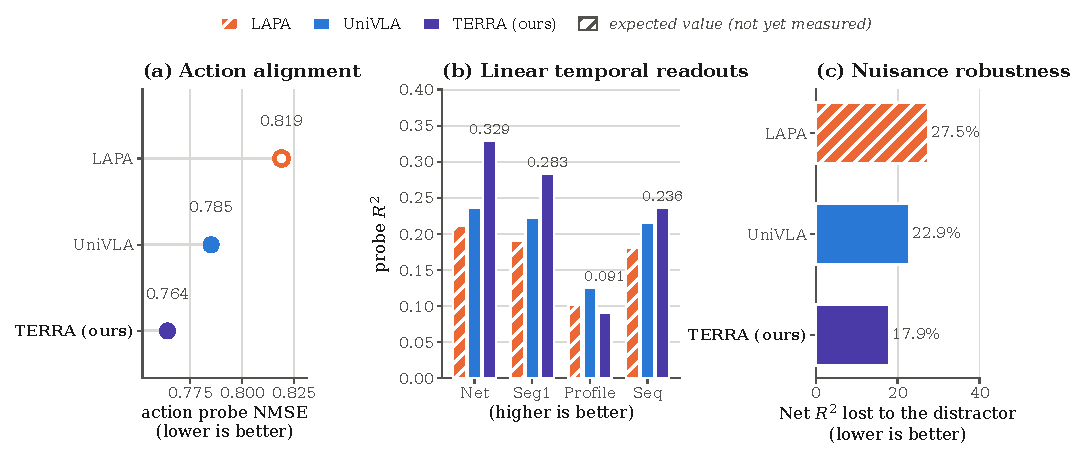
\includegraphics[width=\textwidth]
    {figures/representation_comparison.pdf}
    \caption{
    \textbf{Temporal Effect Representation preserves useful transition
    structure while remaining robust to nuisance variation.}
    All tokenizers are frozen and read the same cached visual features.
    \textbf{(a)} Linear action probe; lower NMSE indicates stronger action
    alignment.
    \textbf{(b)} Linear temporal readouts, showing which accumulated and
    within-window transition information stays linearly accessible.
    \textbf{(c)} Relative degradation of Net $R^2$ under the moving-patch
    distractor; lower is better.
    }
    \label{fig:representation_comparison}
\end{figure}

TERRA attains the strongest action alignment of the three tokenizers and the
highest linear temporal readout on the accumulated, segment-level, and
full-sequence targets.
Against the matched UniVLA baseline it improves the accumulated (Net) and
first-segment (Seg1) readouts by .093 and .061 respectively, and it reduces
distractor-induced degradation from 22.9\% to 17.9\%.
% Repo values (LEDGER 2026-09-14 / 09-16), which the figure currently draws:
%   Net .329 vs .236, Seg1 .283 vs .222, Seq .236 vs .215  -> ours ahead
%   Profile .091 vs .125                                   -> ours behind
% The sentence below matches that figure. When the updated Profile number lands,
% change the one line in acdc_la/figures/make_paper_figures.py and swap in:
%   "The within-window profile follows the same ordering, so the improvement is
%    not a trade of one temporal aspect against another."
The within-window profile is the one target on which the matched baseline
stays ahead (.125 vs .091), indicating that the two methods allocate
accessible temporal information differently rather than following a single
scalar ordering.

The action probe provides the cross-method measure of action alignment,
whereas the temporal readouts diagnose which aspects of the transition remain
linearly accessible, and the distractor sweep separates accessible action
content from sensitivity to motion that carries no action information.

\paragraph{The temporal factorization is what produces this.}
Existing latent-action models derive the latent from a \emph{pair} of frames.
Over a window of $K$ consecutive feature differences, that construction is
exactly the endpoint difference, which is also what pooling the window
returns:
\begin{equation}
\frac{1}{K}\sum_{k=1}^{K}\Delta F_k
\;=\;\frac{1}{K}\bigl(F_{T}-F_{0}\bigr).
\label{eq:endpoint_identity}
\end{equation}
The control in Figure~\ref{fig:temporal_ablation} is therefore not an
arbitrary pooling choice: it is the standard frame-pair treatment, trained in
our architecture on the same data, budget, decoder, and probe, so that the
only difference from TERRA is whether the within-window ordering is kept.
Replacing the factorized temporal effect with this endpoint code leaves the
accumulated readout essentially unchanged (Net .336 vs .329) but removes
almost all within-window structure (Profile .017 vs .091, Seg1 .210 vs .283)
and nearly doubles the loss caused by the distractor (33.6\% vs 17.9\%).
An endpoint code preserves where the window ends up while discarding how it
got there.
This is a statement about a \emph{window-level} code, not about frame-pair
models in general: a pair encoder re-applied at a finer stride, as in UniVLA,
emits one code per segment and does not discard the temporal axis; that
regime is the comparison of Figure~\ref{fig:representation_comparison}.

\begin{figure}[t]
    \centering
    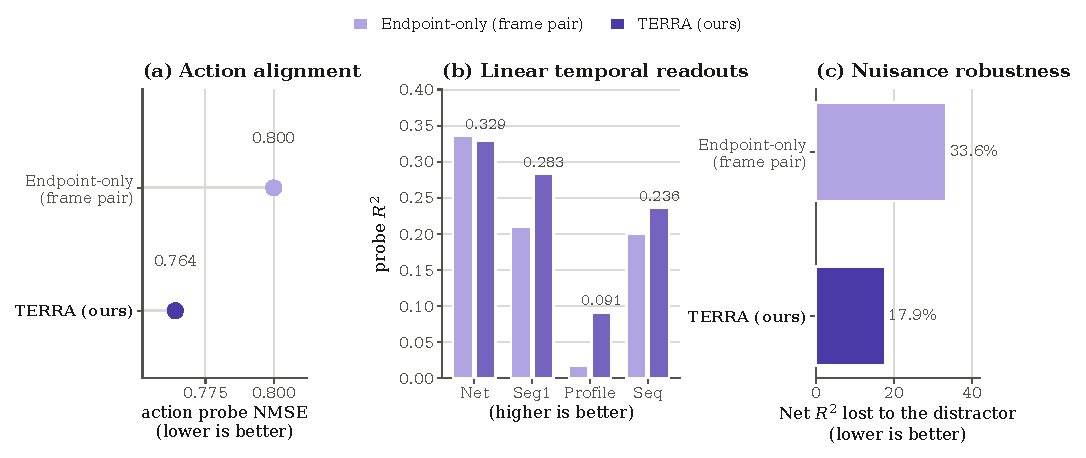
\includegraphics[width=0.78\textwidth]
    {figures/representation_ablation.pdf}
    \caption{
    \textbf{What the temporal factorization buys.}
    Same tokenizer family, data, budget, and probe; only the temporal operator
    changes.
    The endpoint code of Eq.~\ref{eq:endpoint_identity}, the treatment used by
    frame-pair latent-action models, retains the accumulated displacement
    \textbf{(a)} but loses within-window structure and is markedly more
    sensitive to the distractor \textbf{(b)}.
    }
    \label{fig:temporal_ablation}
\end{figure}


\subsection{Relational Alignment via EAT}
\label{sec:eat_results}

We next isolate the effect of relational alignment from additional
optimization.
All continuation runs start from the same 65k-step representation checkpoint
and receive the same 15k-step additional training budget with the same
learning-rate schedule.
Self-reconstruction is retained throughout refinement.
Figure~\ref{fig:eat_refinement} compares reconstruction-only continuation,
EAT without nuisance invariance, and the complete refinement objective.

\begin{figure}[t]
    \centering
    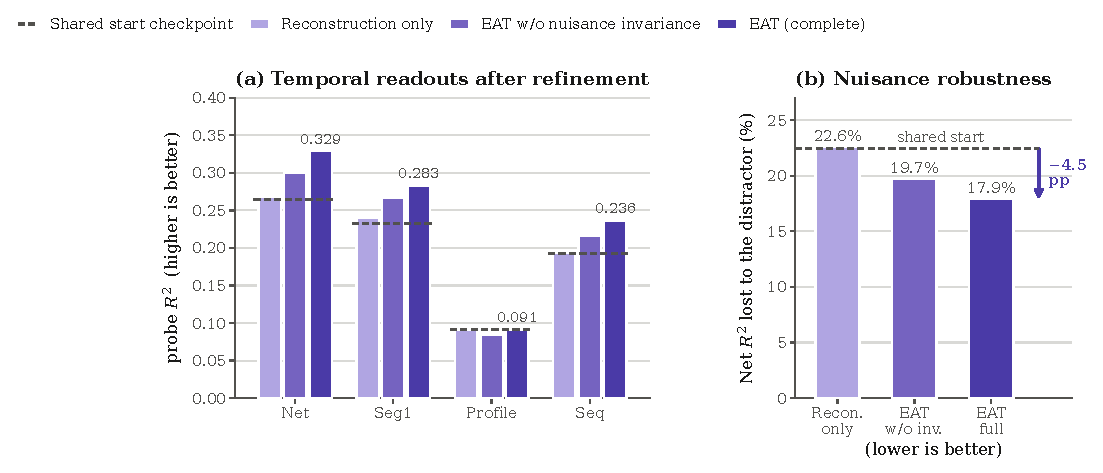
\includegraphics[width=\textwidth]
    {figures/eat_refinement.pdf}
    \caption{
    \textbf{Controlled EAT refinement from a shared representation checkpoint.}
    All continuation variants start from the same checkpoint and use the same
    additional optimization budget; the dashed reference marks that starting
    checkpoint.
    \textbf{(a)} Temporal readouts after refinement.
    \textbf{(b)} Distractor-induced Net degradation.
    Reconstruction-only continuation yields little change, whereas EAT
    improves temporal readout and robustness; nuisance invariance provides an
    additional robustness gain.
    }
    \label{fig:eat_refinement}
\end{figure}

Additional reconstruction alone changes Net $R^2$ only from .265 to .268 and
does not improve distractor robustness.
Under the same continuation budget, EAT raises Net $R^2$ to .300 and lowers
the distractor-induced drop from 22.6\% to 19.7\%.
Adding nuisance invariance further raises Net $R^2$ to .329 and lowers the
drop to 17.9\%.
Relative to reconstruction-only continuation, the complete method improves
Net, Seg1, and Seq readout by .061, .043, and .043, respectively, while
reducing distractor degradation by 4.7 percentage points.
The controlled continuation therefore separates the effect of relational
alignment from simply extending reconstruction training.

Detailed transport diagnostics are reported in
Appendix~\ref{app:transport_analysis}.
These measurements characterize the behavior of the learned transport
operator, but we treat them as supporting diagnostics rather than as
ground-truth measurements of counterfactual physical correctness.


\subsection{Additional Analysis}
\label{sec:additional_analysis}

We place supporting analyses in the appendix to keep the main experimental
story aligned with the two components of TERRA.
These include the spatial-resolution analysis under a fixed readout budget,
cross-context transport diagnostics, interface-specific continuous-VLA
comparisons, checkpoint provenance, and per-task LIBERO results.
 from the main file.
%
% Main-text float budget: one table and three figures.
%   Table~\ref{tab:closed_loop_main}      does the system work in closed loop
%   Fig.~\ref{fig:representation_comparison}  is the representation better than other latent actions
%   Fig.~\ref{fig:temporal_ablation}      does the temporal factorization cause it
%   Fig.~\ref{fig:eat_refinement}         does EAT cause the rest
% Figure files (vector PDF, Type-42 fonts), regenerate all with
%   envs/univla_vla/bin/python -m acdc_la.figures.make_paper_figures
%   figures/representation_comparison.pdf
%   figures/representation_ablation.pdf
%   figures/eat_refinement.pdf
% Not used in the main text: figures/representation_comparison_with_policy.pdf
%   (same probe panels plus a closed-loop panel; kept for a teaser slot or a talk,
%    where it does not sit next to Table~\ref{tab:closed_loop_main}).
% ICLR is single-column: use figure, not figure*.
% =====================================================================

\section{Experiments}
\label{sec:experiments}

\subsection{Experimental Setup}
\label{sec:exp_setup}

\paragraph{Latent-action pretraining.}
We train latent-action models on a matched Open X-Embodiment mixture
containing 29 sources and approximately 8.19M video clips.
Unless otherwise stated, all tokenizers use the same frozen DINOv2 visual
backbone and the same cached visual features.
TERRA first learns the Temporal Effect Representation described in
Section~\ref{sec:temporal_effect_representation} and is then refined with
EAT (Section~\ref{sec:eat}).
The continuous representation contains four 64-dimensional latent slots.
Detailed sampling, augmentation, optimization, and normalization settings
are provided in Appendix~\ref{app:training_details}.

\paragraph{Baselines.}
We compare TERRA with prior latent-action and VLA methods at two levels.
First, we report published LIBERO results to situate TERRA with respect to
established systems.
These numbers follow their original training protocols and are not used for
claims of controlled superiority.
Second, we retrain UniVLA under our data scale and downstream protocol for
a direct matched-scale comparison.
For representation analysis we additionally probe the released LAPA
tokenizer, and use an endpoint (frame-pair) tokenizer and a
reconstruction-only continuation as controlled internal references.
% CHECK: the LAPA probe row of Fig.~\ref{fig:representation_comparison} is a
% placeholder (.212/.191/.102/.181, drop 27.5%). Either measure it before
% submission or drop LAPA from the figure and keep it only in
% Table~\ref{tab:closed_loop_main}.
The locally trained UniVLA Stage-2 model follows the official recipe and
inherits the released Stage-1 task-irrelevant prior; we report this
provenance explicitly and analyze its effect in the appendix.

\paragraph{Policy adaptation and evaluation.}
The downstream pipeline follows UniVLA.
Both arms first run the latent-action VLM pretraining stage on 10\% of the
pretraining mixture, an identical budget, and are then fine-tuned on LIBERO
with UniVLA's downstream configuration; the policy is initialized from
OpenVLA-7B.
Our continuous models use the post-instruction query interface and
continuous action expert described in Appendix~\ref{app:vla_adaptation}.
Only the latent labeller differs between the two arms.
Closed-loop success rate is the primary downstream metric.
Each suite contains 10 tasks and is evaluated with 50 rollouts per task.

\paragraph{Representation analysis.}
For latent quality, we follow prior work and use a frozen-tokenizer linear
action probe with normalized mean-squared error (NMSE) as the primary
action-alignment measure~\citep{lee2026why}.
We additionally use temporal readouts and controlled distractors to examine
which transition information is retained and how robustly it is represented.
Every tokenizer is frozen, reads the same cached visual features, and is
evaluated with the same probe protocol, so the comparison isolates the
representation rather than the readout.
Metric definitions and probe architectures are given in
Appendix~\ref{app:metrics}.


\subsection{Closed-loop Manipulation}
\label{sec:closed_loop}

We first evaluate the complete system in closed-loop manipulation.
Table~\ref{tab:closed_loop_main} separates published results under their
original training protocols from our controlled matched-scale comparison.
Only the lower block is used for direct comparison.

\begin{table}[t]
\caption{
\textbf{Closed-loop success rate (\%) on LIBERO.}
Published results are reported under their original training protocols and
serve only as context.
The lower block is our direct comparison: both arms run the latent-action
VLM pretraining stage on 10\% of the mixture and are then fine-tuned with the
same downstream recipe, so only the latent labeller differs.
}
\label{tab:closed_loop_main}
\centering
\footnotesize
\setlength{\tabcolsep}{3.6pt}
\begin{tabular}{lccccc}
\toprule
Method & Spatial & Object & Goal & Long & Avg. \\
\midrule
\multicolumn{6}{l}{\textit{Published results under original protocols}} \\
LAPA             & 73.8 & 74.6 & 58.8 & 55.4 & 65.7 \\
Diffusion Policy & 78.3 & 92.5 & 68.3 & 50.5 & 72.4 \\
Octo             & 78.9 & 85.7 & 84.6 & 51.1 & 75.1 \\
OpenVLA          & 84.7 & 88.4 & 79.2 & 53.7 & 76.5 \\
UniVLA           & 96.5 & 96.8 & 95.6 & 92.0 & 95.2 \\
\midrule
\multicolumn{6}{l}{\textit{Matched pretraining data (10\% of the mixture), identical downstream recipe}} \\
% Measured; reported 2026-09-22. Averages before rounding: UniVLA 91.75, TERRA 93.425 (+1.675).
UniVLA (matched)
& 92.3 & 92.6 & 93.4 & 88.7 & 91.8 \\
\textbf{TERRA (ours)}
& \textbf{94.1} & \textbf{95.2} & \textbf{93.8} & \textbf{90.6}
& \textbf{93.4} \\
\bottomrule
\end{tabular}
\end{table}

Under matched pretraining data, TERRA raises average closed-loop success from
91.8\% to 93.4\%, and is ahead on all four suites: $+1.8$ on Spatial, $+2.6$
on Object, $+0.4$ on Goal, and $+1.9$ on Long.
The gain is largest on Object and Long, the suites that depend most on getting
the intermediate motion right, and smallest on Goal, where both arms are close
to the ceiling of this protocol.
Because this comparison currently uses a single policy fine-tuning seed, we
treat the margin as a system-level result rather than a claim of statistical
significance; with 500 rollouts per suite the standard error is approximately
1.1 points at this success level.
% CHECK: a no-latent control (same backbone, interface and recipe, no latent
% action) has not been run under this protocol and is therefore not in the
% table. It is the control a reviewer will ask for, since it is what separates
% "the latent helps" from "the recipe is good".
Per-task results and additional seeds are reported in the appendix when
available.


\subsection{Temporal Effect Representation}
\label{sec:temporal_repr_results}

We next ask whether the representation of
Section~\ref{sec:temporal_effect_representation} retains useful temporal
structure without becoming unnecessarily sensitive to nuisance variation.
Figure~\ref{fig:representation_comparison} compares frozen latent-action
tokenizers under a single probe protocol: LAPA, UniVLA retrained at our data
scale, and TERRA.
OpenVLA is absent here by construction: it predicts the action directly and
exposes no latent action code to probe, so it enters only the closed-loop
comparison of Table~\ref{tab:closed_loop_main}.

\begin{figure}[t]
    \centering
    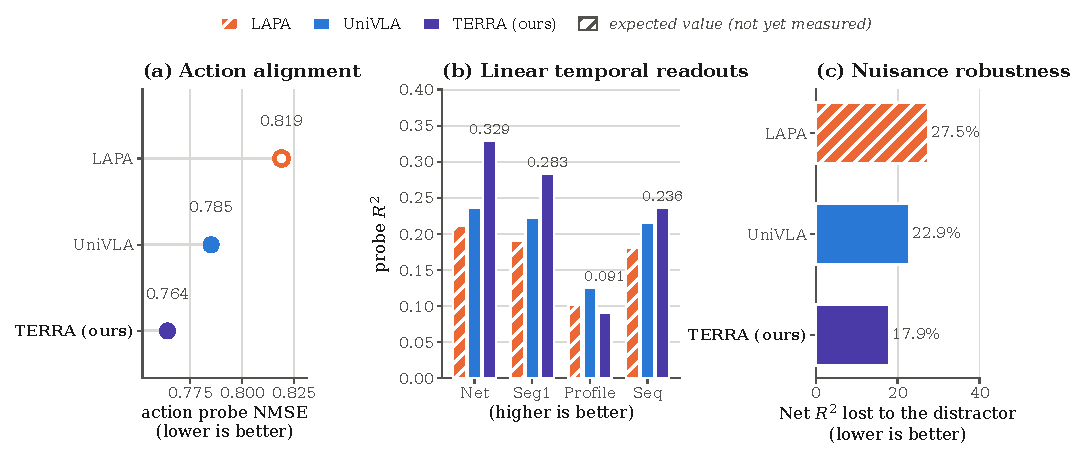
\includegraphics[width=\textwidth]
    {figures/representation_comparison.pdf}
    \caption{
    \textbf{Temporal Effect Representation preserves useful transition
    structure while remaining robust to nuisance variation.}
    All tokenizers are frozen and read the same cached visual features.
    \textbf{(a)} Linear action probe; lower NMSE indicates stronger action
    alignment.
    \textbf{(b)} Linear temporal readouts, showing which accumulated and
    within-window transition information stays linearly accessible.
    \textbf{(c)} Relative degradation of Net $R^2$ under the moving-patch
    distractor; lower is better.
    }
    \label{fig:representation_comparison}
\end{figure}

TERRA attains the strongest action alignment of the three tokenizers and the
highest linear temporal readout on the accumulated, segment-level, and
full-sequence targets.
Against the matched UniVLA baseline it improves the accumulated (Net) and
first-segment (Seg1) readouts by .093 and .061 respectively, and it reduces
distractor-induced degradation from 22.9\% to 17.9\%.
% Repo values (LEDGER 2026-09-14 / 09-16), which the figure currently draws:
%   Net .329 vs .236, Seg1 .283 vs .222, Seq .236 vs .215  -> ours ahead
%   Profile .091 vs .125                                   -> ours behind
% The sentence below matches that figure. When the updated Profile number lands,
% change the one line in acdc_la/figures/make_paper_figures.py and swap in:
%   "The within-window profile follows the same ordering, so the improvement is
%    not a trade of one temporal aspect against another."
The within-window profile is the one target on which the matched baseline
stays ahead (.125 vs .091), indicating that the two methods allocate
accessible temporal information differently rather than following a single
scalar ordering.

The action probe provides the cross-method measure of action alignment,
whereas the temporal readouts diagnose which aspects of the transition remain
linearly accessible, and the distractor sweep separates accessible action
content from sensitivity to motion that carries no action information.

\paragraph{The temporal factorization is what produces this.}
Existing latent-action models derive the latent from a \emph{pair} of frames.
Over a window of $K$ consecutive feature differences, that construction is
exactly the endpoint difference, which is also what pooling the window
returns:
\begin{equation}
\frac{1}{K}\sum_{k=1}^{K}\Delta F_k
\;=\;\frac{1}{K}\bigl(F_{T}-F_{0}\bigr).
\label{eq:endpoint_identity}
\end{equation}
The control in Figure~\ref{fig:temporal_ablation} is therefore not an
arbitrary pooling choice: it is the standard frame-pair treatment, trained in
our architecture on the same data, budget, decoder, and probe, so that the
only difference from TERRA is whether the within-window ordering is kept.
Replacing the factorized temporal effect with this endpoint code leaves the
accumulated readout essentially unchanged (Net .336 vs .329) but removes
almost all within-window structure (Profile .017 vs .091, Seg1 .210 vs .283)
and nearly doubles the loss caused by the distractor (33.6\% vs 17.9\%).
An endpoint code preserves where the window ends up while discarding how it
got there.
This is a statement about a \emph{window-level} code, not about frame-pair
models in general: a pair encoder re-applied at a finer stride, as in UniVLA,
emits one code per segment and does not discard the temporal axis; that
regime is the comparison of Figure~\ref{fig:representation_comparison}.

\begin{figure}[t]
    \centering
    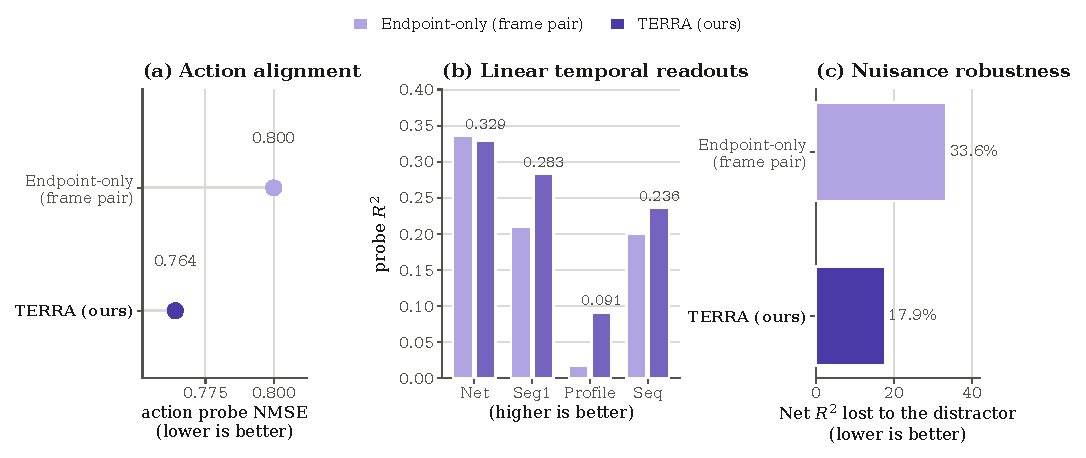
\includegraphics[width=0.78\textwidth]
    {figures/representation_ablation.pdf}
    \caption{
    \textbf{What the temporal factorization buys.}
    Same tokenizer family, data, budget, and probe; only the temporal operator
    changes.
    The endpoint code of Eq.~\ref{eq:endpoint_identity}, the treatment used by
    frame-pair latent-action models, retains the accumulated displacement
    \textbf{(a)} but loses within-window structure and is markedly more
    sensitive to the distractor \textbf{(b)}.
    }
    \label{fig:temporal_ablation}
\end{figure}


\subsection{Relational Alignment via EAT}
\label{sec:eat_results}

We next isolate the effect of relational alignment from additional
optimization.
All continuation runs start from the same 65k-step representation checkpoint
and receive the same 15k-step additional training budget with the same
learning-rate schedule.
Self-reconstruction is retained throughout refinement.
Figure~\ref{fig:eat_refinement} compares reconstruction-only continuation,
EAT without nuisance invariance, and the complete refinement objective.

\begin{figure}[t]
    \centering
    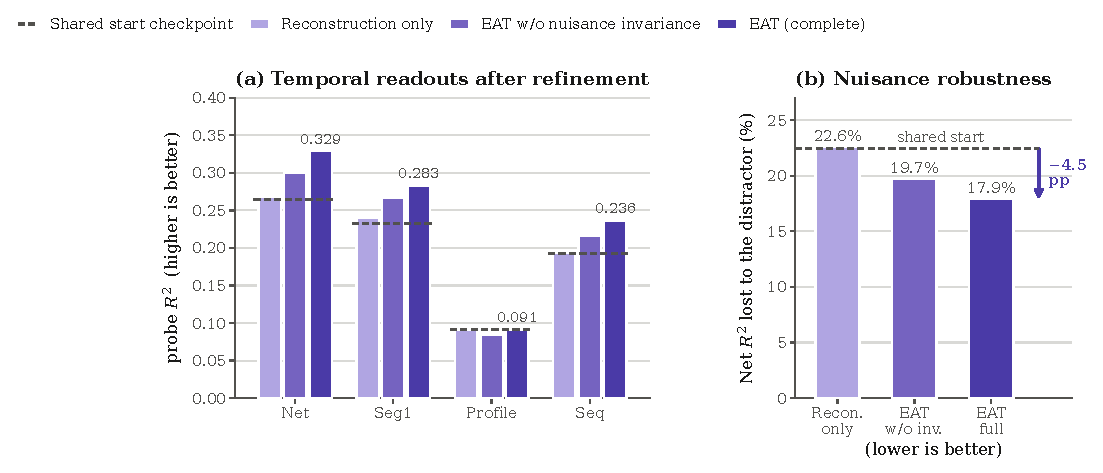
\includegraphics[width=\textwidth]
    {figures/eat_refinement.pdf}
    \caption{
    \textbf{Controlled EAT refinement from a shared representation checkpoint.}
    All continuation variants start from the same checkpoint and use the same
    additional optimization budget; the dashed reference marks that starting
    checkpoint.
    \textbf{(a)} Temporal readouts after refinement.
    \textbf{(b)} Distractor-induced Net degradation.
    Reconstruction-only continuation yields little change, whereas EAT
    improves temporal readout and robustness; nuisance invariance provides an
    additional robustness gain.
    }
    \label{fig:eat_refinement}
\end{figure}

Additional reconstruction alone changes Net $R^2$ only from .265 to .268 and
does not improve distractor robustness.
Under the same continuation budget, EAT raises Net $R^2$ to .300 and lowers
the distractor-induced drop from 22.6\% to 19.7\%.
Adding nuisance invariance further raises Net $R^2$ to .329 and lowers the
drop to 17.9\%.
Relative to reconstruction-only continuation, the complete method improves
Net, Seg1, and Seq readout by .061, .043, and .043, respectively, while
reducing distractor degradation by 4.7 percentage points.
The controlled continuation therefore separates the effect of relational
alignment from simply extending reconstruction training.

Detailed transport diagnostics are reported in
Appendix~\ref{app:transport_analysis}.
These measurements characterize the behavior of the learned transport
operator, but we treat them as supporting diagnostics rather than as
ground-truth measurements of counterfactual physical correctness.


\subsection{Additional Analysis}
\label{sec:additional_analysis}

We place supporting analyses in the appendix to keep the main experimental
story aligned with the two components of TERRA.
These include the spatial-resolution analysis under a fixed readout budget,
cross-context transport diagnostics, interface-specific continuous-VLA
comparisons, checkpoint provenance, and per-task LIBERO results.
